\chapter{研究方法}
\label{cha:experiment}

\section{应用功能设计}
\label{sec:app_design}
\begin{figure}[h]
	\centering
	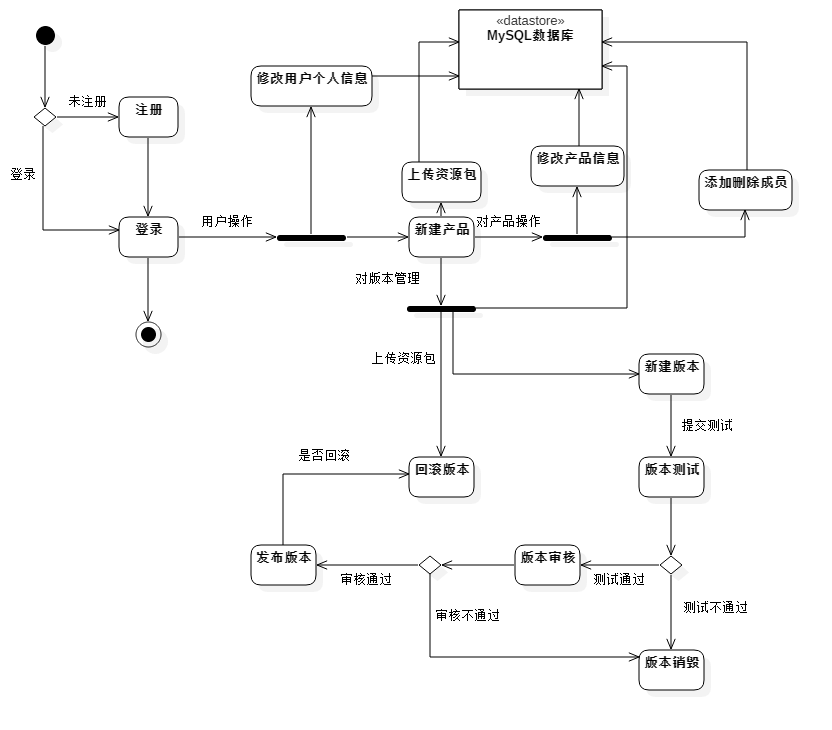
\includegraphics[width=0.5\textwidth]{image/UML/ActivityDiagram.png}
	\caption{应用功能设计}
	\label{fig:app}
\end{figure}
\section{前端架构}
\label{sec:Front-end_architecture}

\section{界面设计}
\label{sec:UI}
阿里巴巴针对angular封装了对应的UI风格和许多实用的组件供开发者使用,让开发者不必花费过多的时间在UI的设计上面,让开发的周期变得更短。

使用方法:npm install ng-zorro-antd
\section{数据库设计}
\label{sec:database_design}
\begin{figure}[h]
	\centering
	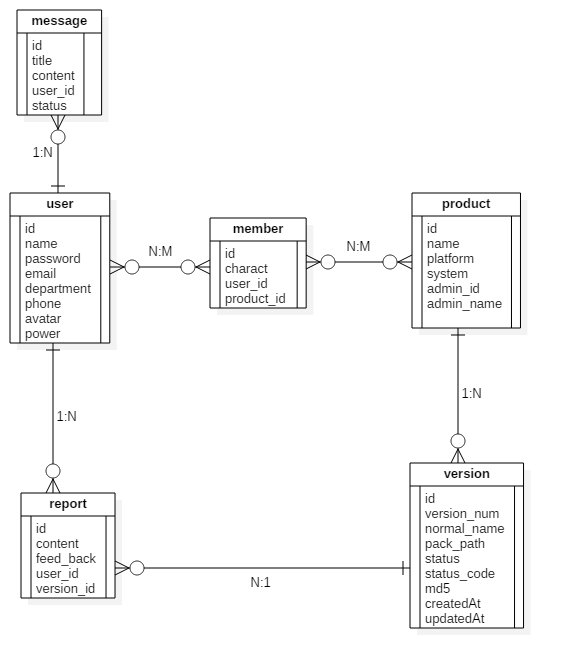
\includegraphics[width=0.5\textwidth]{image/UML/ERDDiagram.png}
	\caption{数据库设计}
	\label{fig:database}
\end{figure}
\section{后端开发}
\label{sec:Backend_development }
dd